\apendice{Especificación de Requisitos}

\section{Diagrama de casos de uso}

Figura \ref{fig:diagrama_casos_uso}.

\begin{figure}[h]
    \centering
    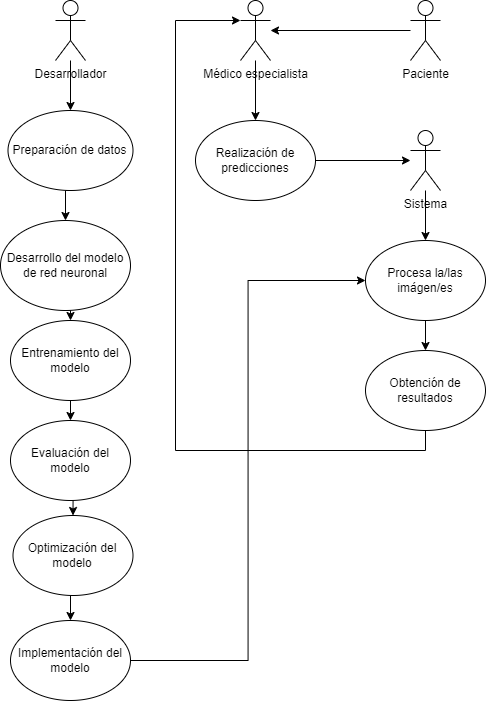
\includegraphics[width=0.99\textwidth]{img/diagrama_casos_uso.PNG}
    \caption{Diagrama de casos de uso realizado con draw.io. Fuente propia.}
    \label{fig:diagrama_casos_uso}
\end{figure}
\FloatBarrier

\section{Explicación casos de uso.}

En este trabajo se ha desarrollado un diagrama de casos de uso \ref{fig:diagrama_casos_uso} que incluye como actores al desarrollador o programador, el neumólogo especializado, el paciente y el sistema. Aunque el enfoque principal de este trabajo ha sido el desarrollo del modelo de red neuronal por parte del desarrollador, se han incluido los casos de uso de los otros actores para ilustrar el potencial y las aplicaciones futuras del proyecto en el ámbito médico.

\subsection{Desarrollador}
El desarrollador es la persona que desarrolla y ajusta el modelo de red neuronal. Sus casos de uso son los siguientes:
\begin{itemize}
    \item \textbf{Preparación de los datos} que incluye tanto la recopilación de imágenes de CXT con y sin neumonía como el preprocesamiento de las imágenes.
    \item \textbf{Desarrollo del modelo de red neuronal} se refiere tanto al desarrollo de la arquitectura de la red neuronal inicial como a los hiperparámetros empleados inicialmente.
    \item \textbf{Entrenamiento del modelo} a partir de las imágenes etiquetadas y su correspondiente validación. También se realiza el ajuste de hiperparámetros según los resultados de validación.
    \item \textbf{Evaluación del rendimiento del modelo} a partir del conjunto de prueba (o test). Para la evaluación del modelo se emplean una serie de métricas como \textit{accuracy}, \textit{recall}, \textit{precision}, AUC, etc.
    \item \textbf{Optimización del modelo} a partir del ajuste de distintos hiperparámetros y reentrenamiento del modelo hasta obtener el idóneo.
    \item \textbf{Implementación del modelo} en un ambiente operativo
\end{itemize}

\subsection{Médico especialista, paciente y sistema}
Como ya se ha comentado en el apartado de ``Líneas futuras'' de la memoria, el objetivo tanto de este trabajo como de otros similares ya realizados es su introducción en el ámbito clínico, aunque, para eso aún son necesarias algunas mejoras. 

Aun así, se ha diseñado también la parte de diagrama de casos de uso llevado al ámbito clínico el cuál se explica a continuación:

\begin{enumerate}
    \item El paciente acude a la consulta con el neumólogo
    \item El médico especializado le realiza una CXT 
    \item Esta imagen es introducida en el sistema previamente desarrollado, el cual es capaz de identificar en esa imagen la presencia o ausencia de neumonía
    \item El sistema muestra en la pantalla del médico si se trata de una neumonía o no
\end{enumerate}



